%%%%%%%%%%%%%%%%%%%%%%%%%%%%%%%%%%%%%%%%%
% Beamer Presentation
% LaTeX Template
% Version 1.0 (10/11/12)
%
% This template has been downloaded from:
% http://www.LaTeXTemplates.com
%
% License:
% CC BY-NC-SA 3.0 (http://creativecommons.org/licenses/by-nc-sa/3.0/)
%
%%%%%%%%%%%%%%%%%%%%%%%%%%%%%%%%%%%%%%%%%

%----------------------------------------------------------------------------------------
%	PACKAGES AND THEMES
%----------------------------------------------------------------------------------------

\documentclass{beamer}

\mode<presentation> {
	
	% The Beamer class comes with a number of default slide themes
	% which change the colors and layouts of slides. Below this is a list
	% of all the themes, uncomment each in turn to see what they look like.
	
	%\usetheme{default}
	%\usetheme{AnnArbor}
	%\usetheme{Antibes}
	%\usetheme{Bergen}
	%\usetheme{Berkeley}
	%\usetheme{Berlin}
	%\usetheme{Boadilla}
	%\usetheme{CambridgeUS}
	%\usetheme{Copenhagen}
	%\usetheme{Darmstadt}
	%\usetheme{Dresden}
	%\usetheme{Frankfurt}
	%\usetheme{Goettingen}
	%\usetheme{Hannover}
	%\usetheme{Ilmenau}
	%\usetheme{JuanLesPins}
	%\usetheme{Luebeck}
	\usetheme{Madrid}
	%\usetheme{Malmoe}
	%\usetheme{Marburg}
	%\usetheme{Montpellier}
	%\usetheme{PaloAlto}
	%\usetheme{Pittsburgh}
	%\usetheme{Rochester}
	%\usetheme{Singapore}
	%\usetheme{Szeged}
	%\usetheme{Warsaw}
	
	% As well as themes, the Beamer class has a number of color themes
	% for any slide theme. Uncomment each of these in turn to see how it
	% changes the colors of your current slide theme.
	
	%\usecolortheme{albatross}
	\usecolortheme{beaver}
	%\usecolortheme{beetle}
	%\usecolortheme{crane}
	%\usecolortheme{dolphin}
	%\usecolortheme{dove}
	%\usecolortheme{fly}
	%\usecolortheme{lily}
	%\usecolortheme{orchid}
	%\usecolortheme{rose}
	%\usecolortheme{seagull}
	%\usecolortheme{seahorse}
	%\usecolortheme{whale}
	%\usecolortheme{wolverine}
	
	%\setbeamertemplate{footline} % To remove the footer line in all slides uncomment this line
	%\setbeamertemplate{footline}[page number] % To replace the footer line in all slides with a simple slide count uncomment this line
	
	%\setbeamertemplate{navigation symbols}{} % To remove the navigation symbols from the bottom of all slides uncomment this line
}

\usepackage{graphicx} % Allows including images
\usepackage{subfigure}
\usepackage{booktabs} % Allows the use of \toprule, \midrule and \bottomrule in tables
\usepackage{bm}

%----------------------------------------------------------------------------------------
%	TITLE PAGE
%----------------------------------------------------------------------------------------

\title[multi-ridge]{Dimension Reduction and Coefficient Estimation in Multivariate Linear Regression} 

\author{Ganchao Wei} 
\date{November 17, 2021}

\begin{document}
	
	\begin{frame}
		\titlepage % Print the title page as the first slide
	\end{frame}
	
	\begin{frame}
		\frametitle{Overview} % Table of contents slide, comment this block out to remove it
		\tableofcontents
	\end{frame}
	
	%--------------------------------------------------------------------
	%	PRESENTATION SLIDES
	%--------------------------------------------------------------------
	
	\section{Introduction}
	
	\begin{frame}
		\frametitle{Introduction}
		\textbf{Multivariate linear regression}: 
		$$Y=XB + E$$
		, where $Y\in\mathbb{R}^{n\times q}$, $X\in \mathbb{R}^{n\times p}$ and $B\in \mathbb{R}^{p\times q}$
		To reduce dimension, rewrite the model as the \textbf{linear factor regression}:
		$$Y=XB+E=X\Gamma\Omega + E = F\Omega + E$$
		, where $\Gamma\in\mathbb{R}^{p\times r}$ for some $r\leq \min(p,q)$. The columns of F represent the so-called factors.\\
		\vspace{\baselineskip}
		In this paper, they propose a method simultaneously (1) choose the number of factors, (2) determine the factors and (3) estimate the factor loading $\Omega$.
	\end{frame}
	
	\section{Factor Estimation and Selection}
	
	\begin{frame}
	\frametitle{Factor Estimation and Selection}
	Let $\{\eta_1,\ldots,\eta_p\}$ be a set of basis for $\mathbb{R}^p$. If columns of $B$ come from a linear space $\mathcal{B}\subseteq span\{\eta_i:i\in\mathcal{A}\subset\{1,\ldots,p\}\}$, then we can do dimension reduction.\\
	\vspace{\baselineskip}
	Assume $\{\eta_1,\ldots,\eta_p\}$ are known, let $F = (F_1,\ldots,F_p)$, where $F_i=X\eta_i$, then
	$$Y=F\Omega + E$$
	,where $\Omega\in\mathbb{R}^{p\times q}$, s.t., $\{\eta_1,\ldots,\eta_p\}\Omega = B$. Then the factor selection problem can be reformed as:
	$$\min\{tr\{(Y-F\Omega)W(Y-F\Omega)'\}\}\,\,\text{subject to} \sum_{i=1}^{p}||\omega_i||_{\alpha}\leq t$$
	, where $W$ is a weight matrix (assume $W=I$ in this paper), $\omega_i$ is the $i$th row of $\Omega$, $t\geq 0$ is a regularization parameter and $||\cdot||_{\alpha}$ is the $l_{\alpha}$-norm. (They choose $\alpha = 2$, since the optimization problem is invariant to orthogonal transformation of the response)
	\end{frame}	
	
	\begin{frame}
		\frametitle{Factor Estimation and Selection}
		In this paper, they let $\{\eta_i\}$ be the eigenvectors of $BB'$.\\ 
		\vspace{\baselineskip}
		Denote the SVD of $B$ as $B = UDV'$, where $V\in\mathbb{R}^{p\times p}$. Then columns of U form $\{\eta_i\}$. Further, let $D_{ii} = \sigma_i(B)$ be the $i$th largest singular value. Then $\Omega = DV'$ and $\omega_i=\sigma_i(B)V_i$. Clearly, $||\omega_i||_2 = \sigma_i(B)$ and then the previous objective function can be rewritten as:
		$$\min\{tr\{(Y-XB)(Y-XB)'\}\}\,\,\text{subject to}\sum_{i=1}^{\min(p,q)}\sigma_i(B)\leq t$$
		, where $\sum_{i=1}^{\min(p,q)}\sigma_i(B)$ is the Ky Fan norm of $B$. This is equivalent to a conic program and can be computed efficiently.\\
		\vspace{\baselineskip}
		The proposed method is closely related to other popular methods, such as reduced rank regression (RRR) and ridge regression.
	\end{frame}
	
	\section{Orthogonal Design}
	
	\begin{frame}
		\frametitle{Orthogonal Design}
		To understand further the statistical properties of the method, consider the special case of orthogonal design.
		\begin{figure}
			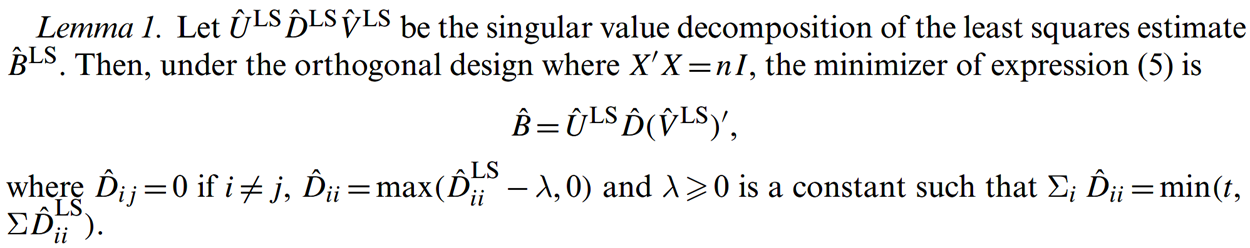
\includegraphics[width=1\linewidth]{image001.png}
		\end{figure}
		Lemma 1 gives an explicit expression for the minimizer.
	\end{frame}
	
	\begin{frame}
		\frametitle{Orthogonal Design}
		The following lemma indicates that we can always find an appropriate tuning parameter such that the non-zero singular values of $B$ are consistently estimated and the rest are set to 0 w.p.1.
		\begin{figure}
			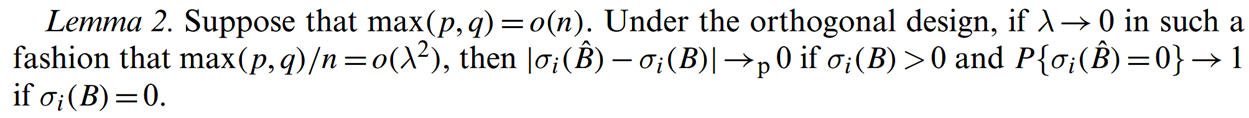
\includegraphics[width=1\linewidth]{image002.png}
		\end{figure}
	\end{frame}
	
	\section{Tuning}
	\begin{frame}
		\frametitle{Tuning}
		\textbf{Tuning parameter}: $t$\\
		Can choose by CV, but is cumbersome. Here, they use GCV type of statistic to determine $t$.\\
		The following lemma explicitly describes the relationship between $t$ and $\lambda$.
		\begin{figure}
			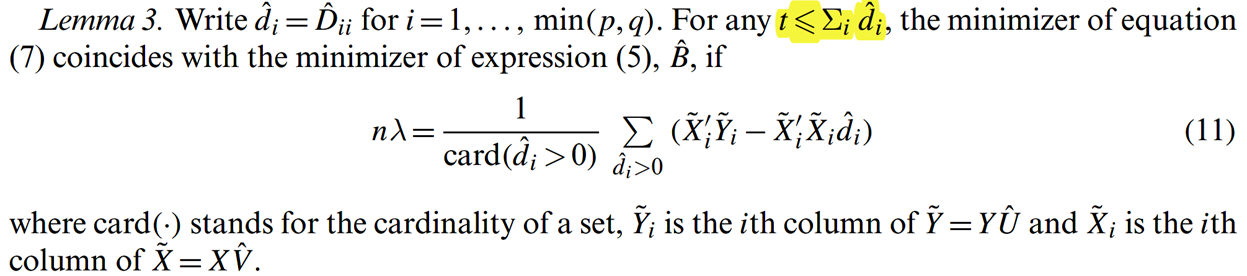
\includegraphics[width=1\linewidth]{image003.png}
		\end{figure}
	\end{frame}
	
	\begin{frame}
		\frametitle{Tuning}
		The minimized $B$ can be expressed as $\hat{B} = (X'X + 2n\lambda K)^{-1}X'Y$ and the GCV score is given by
		$$GCV(t) = \frac{tr\{(Y-X\hat{B})(Y-X\hat{B})'\}}{qp-df(t)}$$\\
		In summary:
		\begin{figure}
			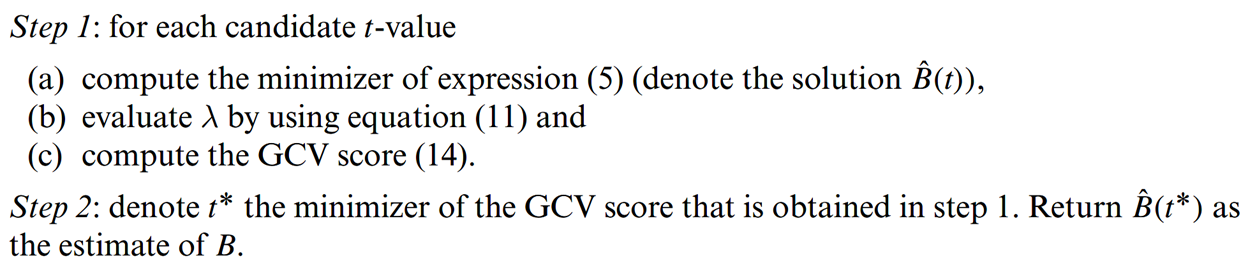
\includegraphics[width=1\linewidth]{image004.png}
		\end{figure}
	\end{frame}
	
	\section{Simulation}
	\begin{frame}
		\frametitle{Simulation}
		The following methods are compared:
		\begin{figure}
			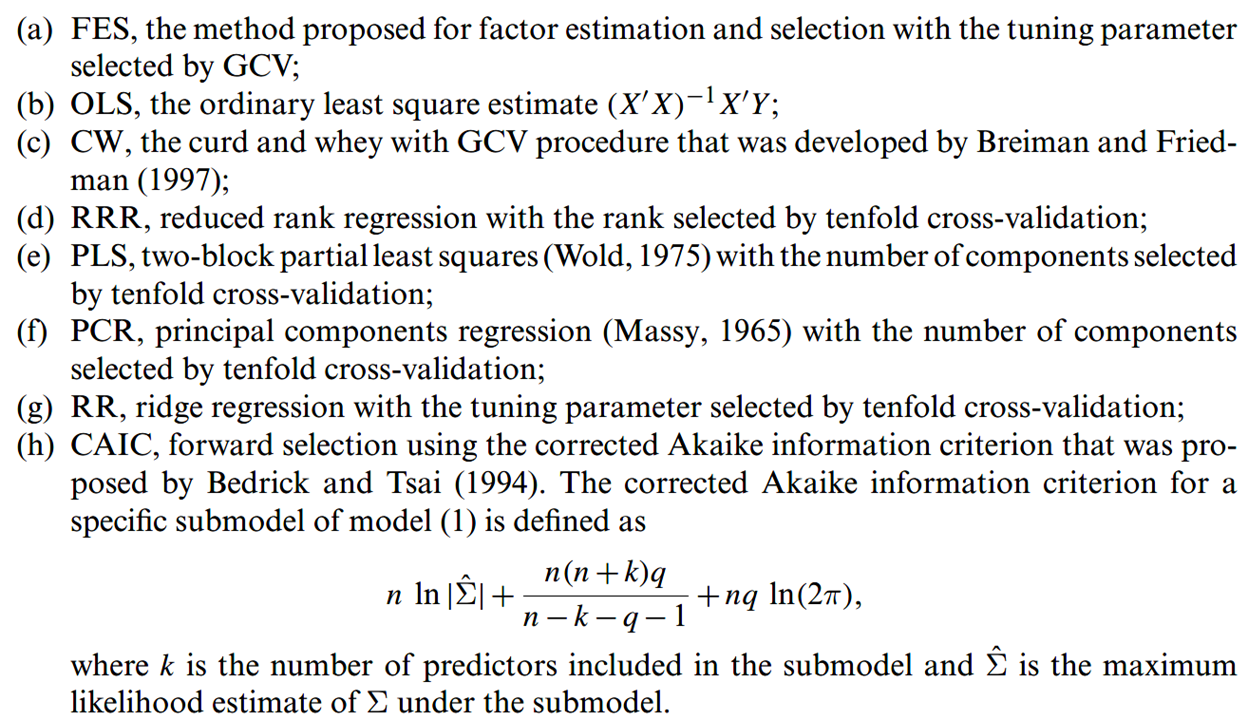
\includegraphics[width=1\linewidth]{image005.png}
		\end{figure}
	\end{frame}
	
	\begin{frame}
		\frametitle{Simulation}
		Comparison is based on the model error $ME(\hat{B})=(\hat{B} - B)'V(\hat{B}-B)$, where $V= E(X'X)$ is the population covariance.\\
		Consider the following 4 models:
		\begin{figure}
			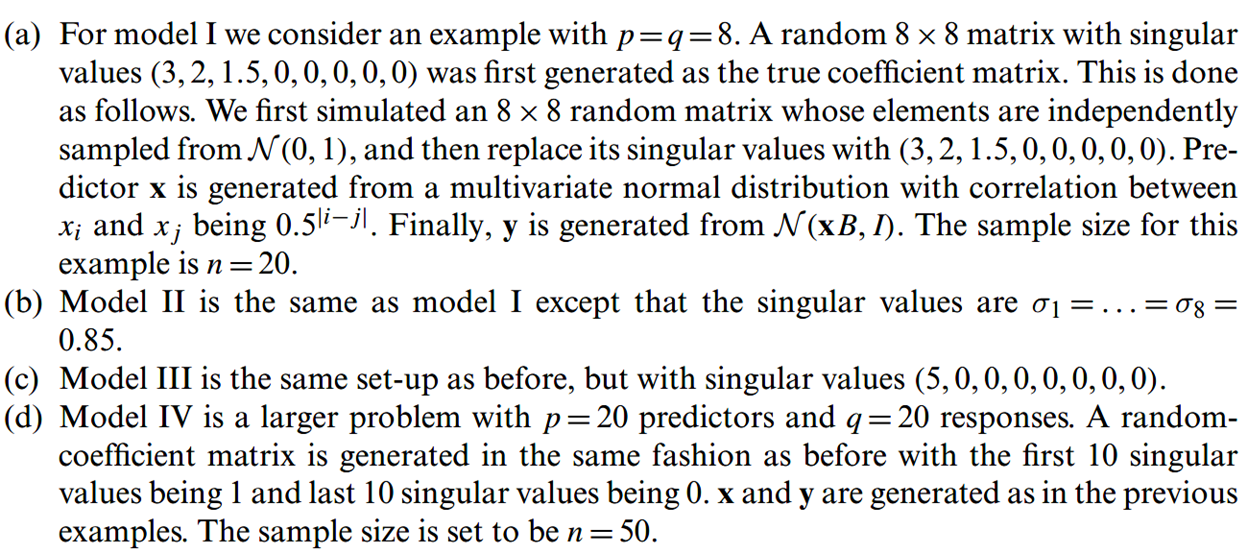
\includegraphics[width=1\linewidth]{image007.png}
		\end{figure}
	\end{frame}
	
	\begin{frame}
		\frametitle{Simulation}
		\begin{figure}
			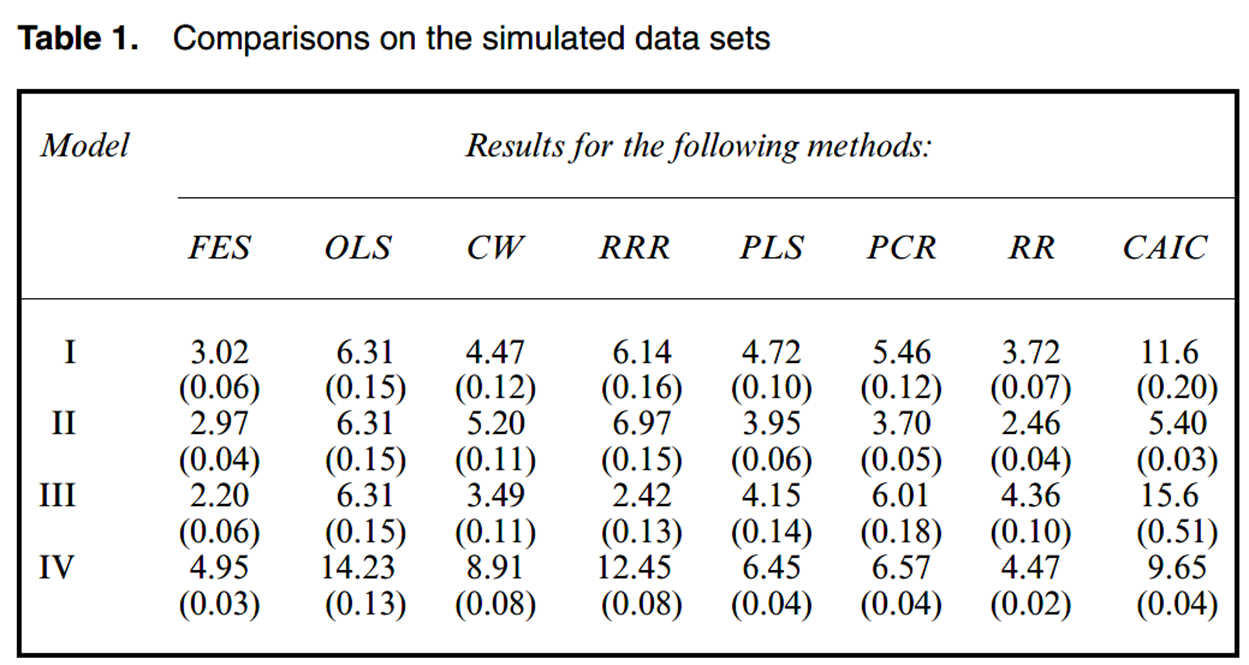
\includegraphics[width=.8\linewidth]{image006.png}
		\end{figure}
	\end{frame}
	
	\begin{frame}
		\frametitle{Simulation}
		\begin{figure}
			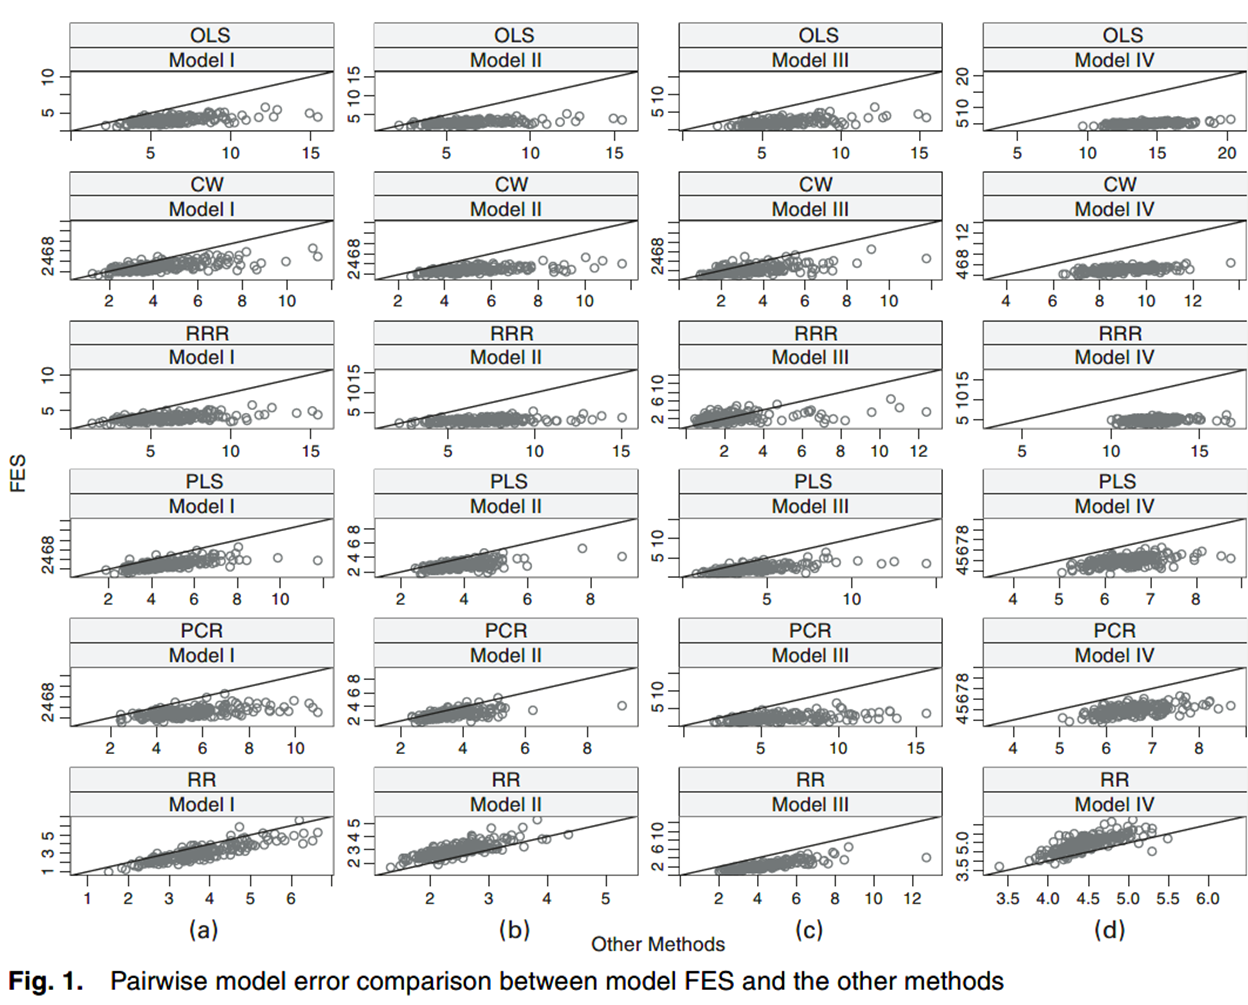
\includegraphics[width=.8\linewidth]{image008.png}
		\end{figure}
	\end{frame}
	
	\section{Application}
	\begin{frame}
		\frametitle{Application}
		The financial data: let $y_t$ be the vector of return at time $t$. The AR(1) model is given by $y_t =y_{t-1}B + E$
		\begin{figure}
			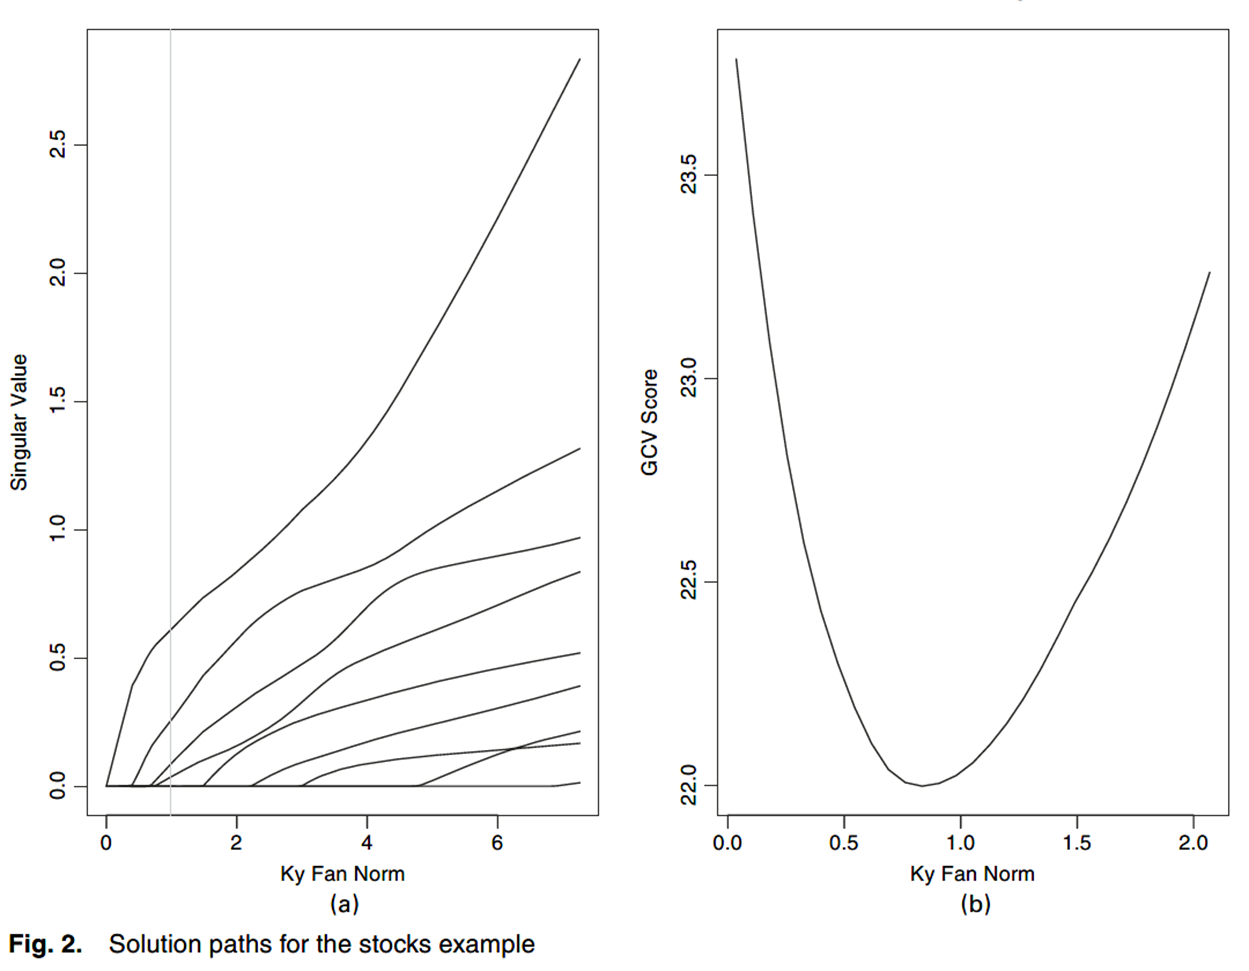
\includegraphics[width=.7\linewidth]{image009.png}
		\end{figure}
	\end{frame}
	
	\begin{frame}
		\frametitle{Application}
		\begin{figure}
			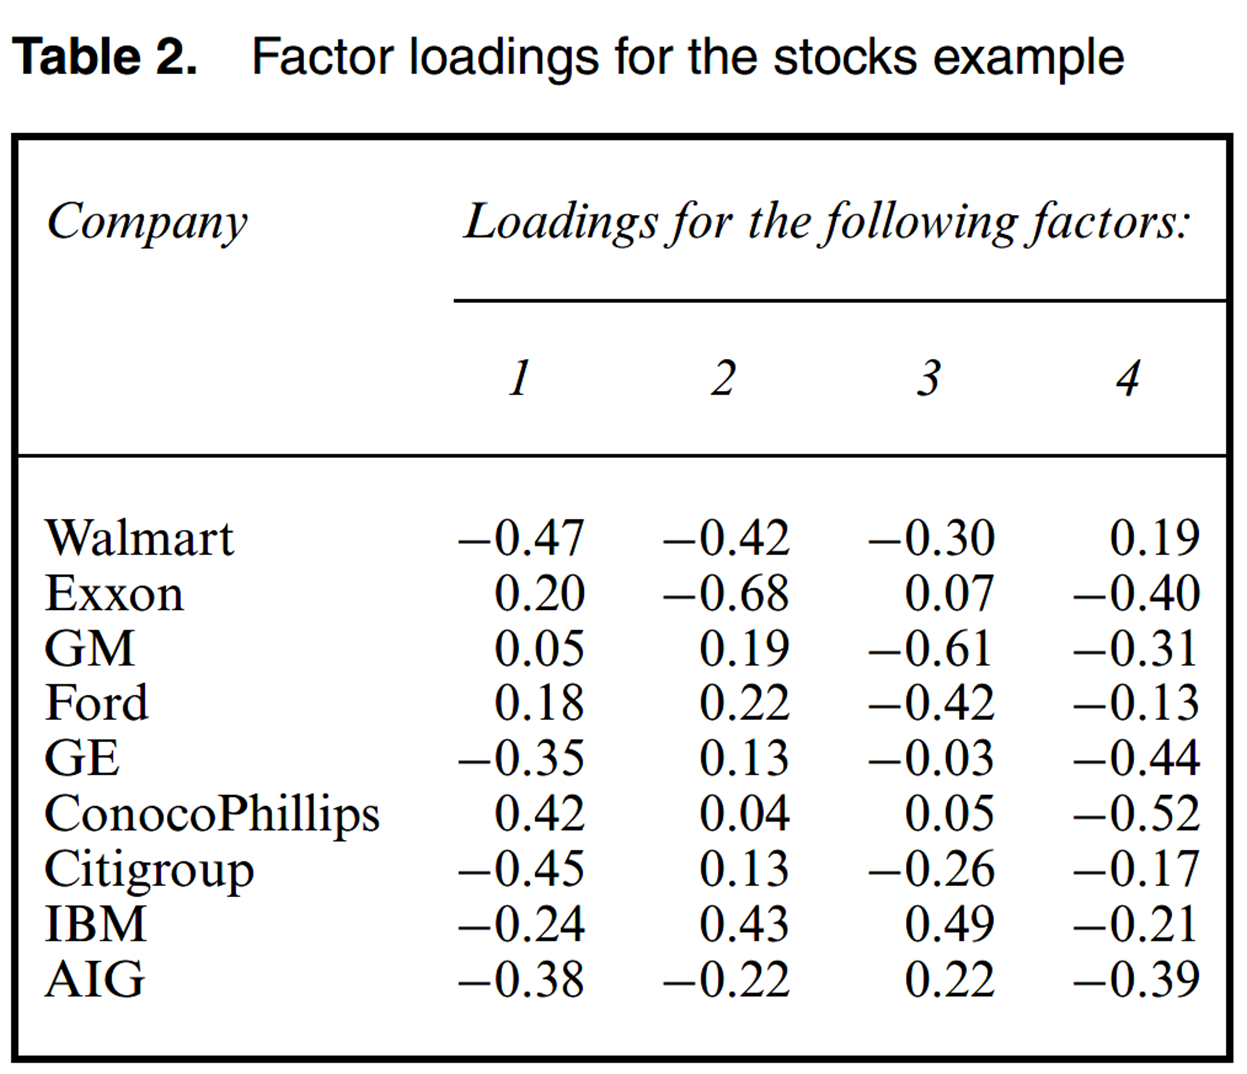
\includegraphics[width=.7\linewidth]{image010.png}
		\end{figure}
	\end{frame}
	
	
	\begin{frame}
		\frametitle{Application}
		\begin{figure}
			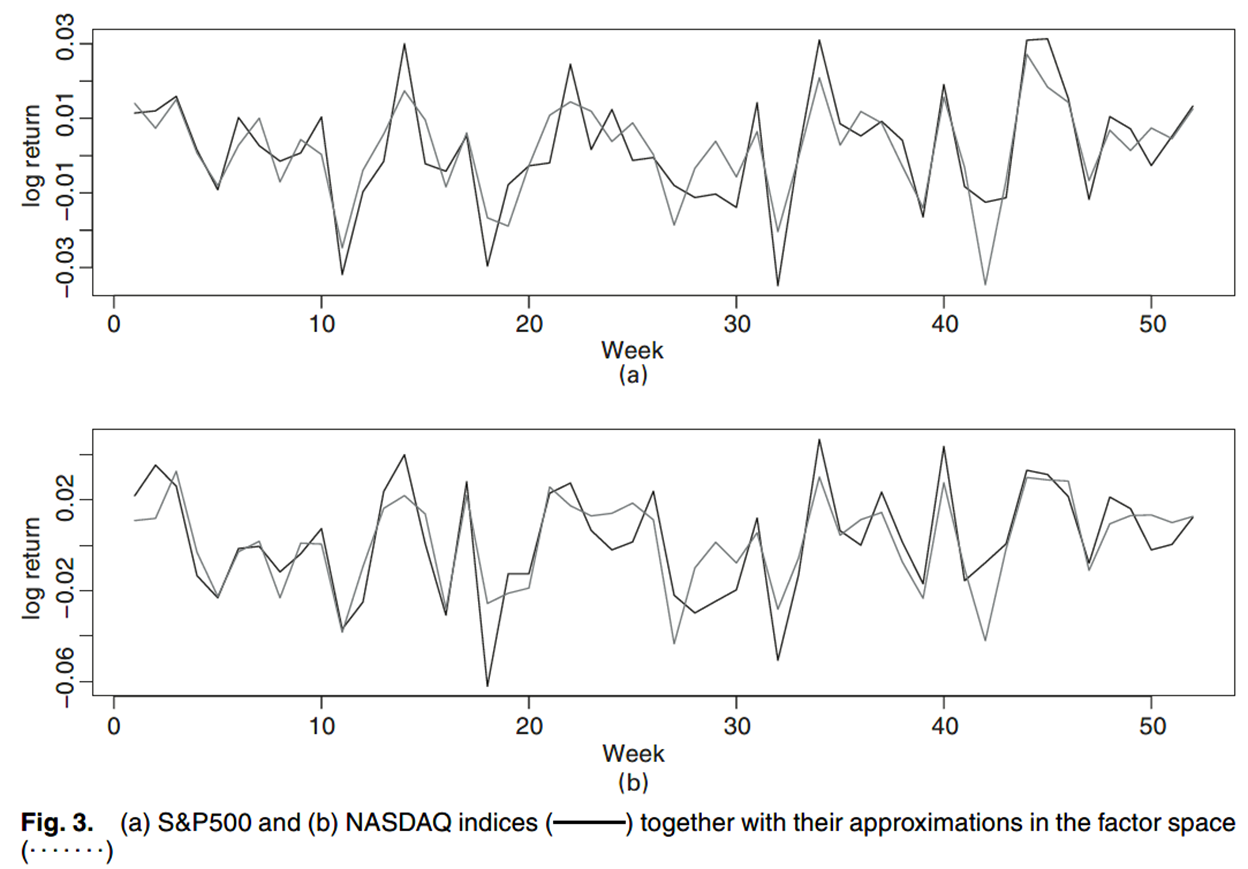
\includegraphics[width=.7\linewidth]{image011.png}
		\end{figure}
	\end{frame}
	
	\begin{frame}
		\frametitle{Application}
		\begin{figure}
			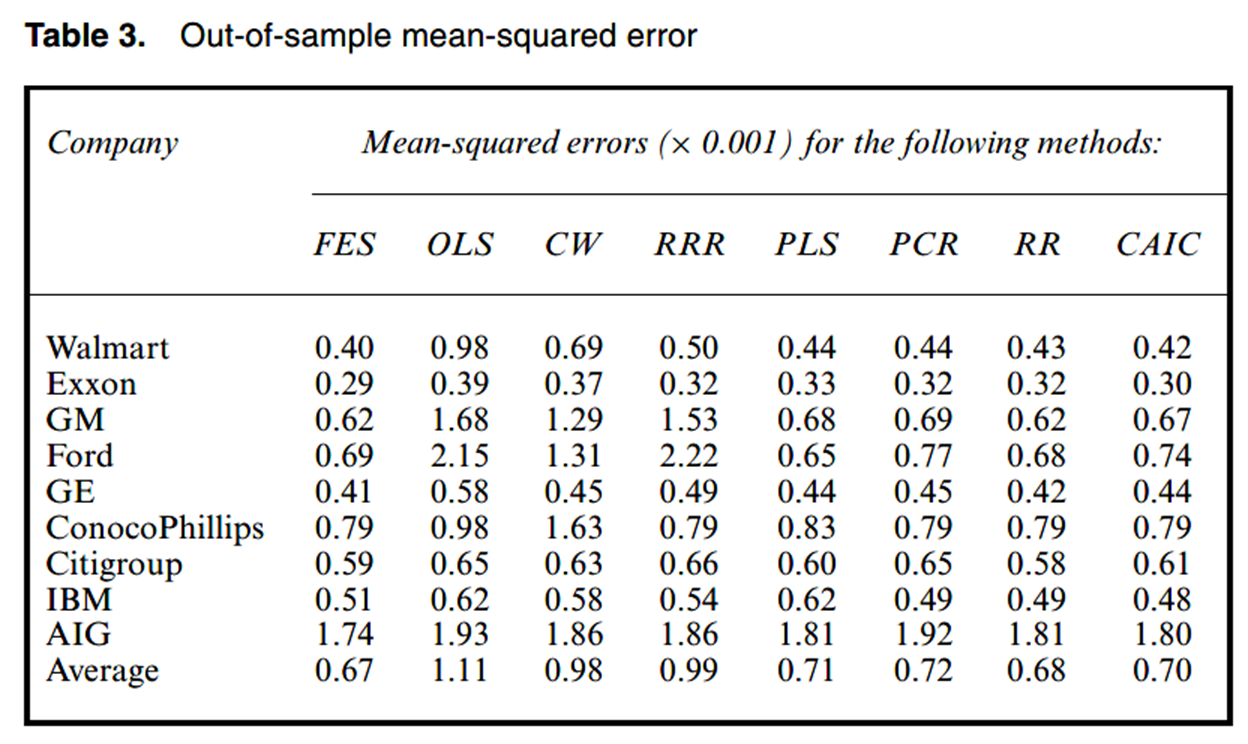
\includegraphics[width=.7\linewidth]{image012.png}
		\end{figure}
	\end{frame}
	
	\section{Non-parametric Factor Model}
	
	\begin{frame}
		\frametitle{Non-parametric actor model}
		By using the penalized spline regression with additive model, we can easily handle the vector non-linear (non-parametric) regression models.\\
		\vspace{\baselineskip}
		This idea is implemented to reanalyse the biochemical data ($n = 33$).\\
		\begin{itemize}
			\item 
			\textbf{5 responses}: pigment creatinine, concentrations of phosphate, phosphorus, creatinine and choline.
			\item
			\textbf{3 predictors}: the weight of the subject, volume and specific gravity.
		\end{itemize}
	\end{frame}
	
	
	\begin{frame}
		\frametitle{Non-parametric actor model}
		\begin{figure}
			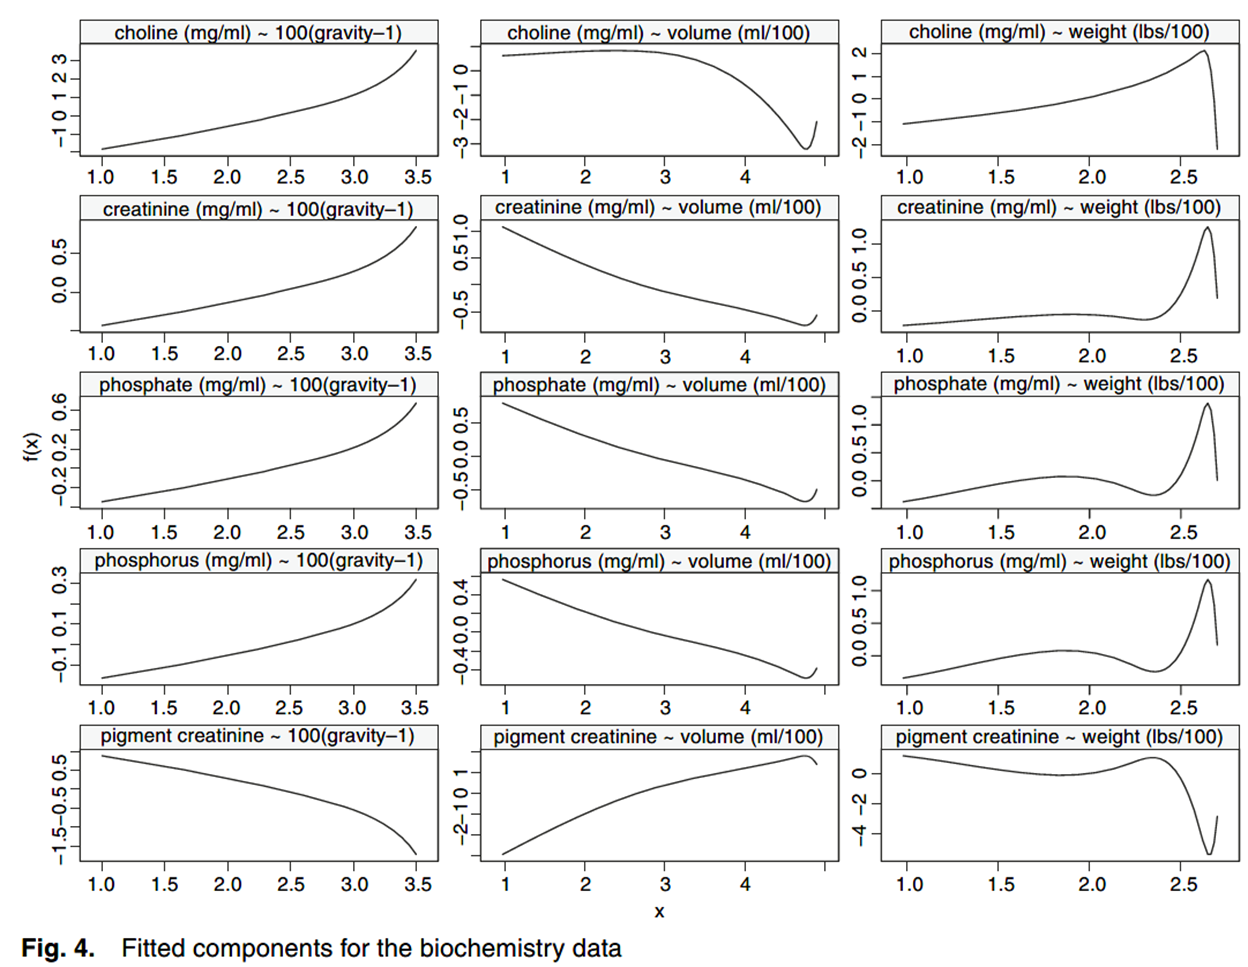
\includegraphics[width=.8\linewidth]{image013.png}
		\end{figure}
	\end{frame}
	
	
\end{document}